\documentclass[11pt,a4paper]{article}
\usepackage{float}
\usepackage{textcomp}
\usepackage{wrapfig}
\usepackage{amsmath}
\usepackage{graphicx}
\usepackage{listings}
\usepackage{enumitem}
\usepackage[dvipsnames]{xcolor}
\usepackage[linktoc=none]{hyperref}
\usepackage[ruled, linesnumbered]{algorithm2e}
\usepackage[justification=centering]{caption}
\usepackage[a4paper, portrait, margin=1.2in]{geometry}
\usepackage[framed, autolinebreaks, useliterate]{mcode}
\hypersetup{
    colorlinks=true,
    linkcolor=blue,
    filecolor=magenta,      
    urlcolor=blue,
}
\lstset{aboveskip=\medskipamount}
\DontPrintSemicolon
\begin{document}
\begin{center}
    \Large\textbf{PageRank}\\
    \vspace{0.2cm}
    \large{Cloud Computing final project - Prof. Nicola Tonellotto}\\
    \vspace{1.0cm}
    \large\textit{Leonardo Turchetti}\\
    \large\textit{Lorenzo Tonelli}\\
    \large\textit{Ludovica Cocchella}\\
    \large\textit{Rambod Rahmani}\\
    \vspace{0.2cm}
    \normalsize{Msc. in Artificial Intelligence and Data Engineering}\\
    \vspace{1.0cm}
    \today
\end{center}
\vspace{1cm}
\tableofcontents
\vspace{1cm}
\section{Introduction}
The importance of a web page is an inherently subjective matter, which depends on the readers interests, knowledge and attitudes. PageRank can be defined as a method for rating web pages objectively and mechanically, effectively measuring the human interest and attention devoted to them. In order to measure the relative importance of web pages, PageRank was proposed as a method for computing a ranking for every web page based on the graph of the web.\\
\\
The project focused on designing a MapReduce algorithm (using pseudocode) to implement the PageRank (using both Hadoop and Spark). Initially, a pseudocode implementation and the design assumptions are presented. The successive sections focus on the implementation details using both Hadoop and Spark. Finally, the validation results obtained using both a realistic and a synthetic dataset are provided.\\
\\
The entire codebase is available at \url{https://github.com/lorytony/CloudComputing}.\\
\\
You can access the VM with the source code ready to be executed using \texttt{ssh hadoop@172.16.3.218} providing the password \texttt{sicurezza34!}. The project files can be found under \texttt{$\sim$/PageRank/hadoop} and \texttt{$\sim$/PageRank/spark}.
\section{PageRank}
PageRank\footnote{The PageRank Citation Ranking: Bringing Order to the Web - January 29, 1998 - \url{http://ilpubs.stanford.edu:8090/422/1/1999-66.pdf}} is a measure of web page quality based on the structure of the hyperlink graph. Although it is only one of thousands of features that is taken into account in Google's search algorithm, it is perhaps one of the best known and most studied. Every page has some number of forward links (out-edges) and backlinks (in-edges). We can never know whether we have found all the backlinks of a particular page but if we have downloaded it, we know all of its forward links at that time.\\
\\
The reason why PageRank is so interesting is that there are many cases where simple citation counting does not correspond to our common sense notion of importance. For example, if a web page has a link off the Yahoo home page, it may be just one link but it is a very important one. This page should be ranked higher than many pages with more links but from obscure places. PageRank is an attempt to see how good an approximation to "importance" can be obtained just from the link structure.\\
\\
The previous example models the so called "Propagation of Ranking Through Links": a page has high rank if the sum of the ranks of its backlinks is high. This covers both the case when a page has many backlinks and when a page has a few highly ranked backlinks.\\
\\
Formally, given
\begin{itemize}
    \item a page $p_i$ among the total $N$ nodes (pages) in the graph;
    \item the set of pages $L(p_i)$ that link to $p_i$;
    \item and the out-degree $C(p_j)$ of node $p_j$;
    \item the random jump factor $\alpha$;
\end{itemize}
the PageRank $PR$ of a page $p_i$ is defined as follows:
$$PR(p_i) = \alpha \frac{1}{N} + (1 - \alpha) \sum_{p_j \in L(p_i)}\frac{PR(p_j)}{C(p_j)}$$
The definition of PageRank above has another intuitive basis in random walks on graphs. The simplified version corresponds to the standing probability distribution of a random walk on the graph of the Web. Intuitively, this can be thought of as modeling the behaviour of a "random surfer". The "random surfer" simply keeps clicking on successive links at random. However, if a real Web surfer ever gets into a small loop of web pages, it is unlikely that the surfer will continue in the loop forever. Instead, the surfer will jump to some other page. The additional factor $\alpha$ can be viewed as a way of modeling this behaviour: the surfer periodically "gets bored" and jumps to a random page.  This residual probability, $\alpha$, is usually set to $0.15$, estimated from the frequency that an average surfer uses his or her browser's bookmark feature. Alternatively, $1 - \alpha$ is referred to as the "damping" factor.
\subsection{Computation}
PageRank can be computed either iteratively or algebraically. Using the iterative method, at $t = 0$, an initial probability distribution is assumed
$$PR(p_i, 0) = \frac{1}{N}$$
where $N$ is the total number of pages, and ($p_i$, $0$) is page $i$ at time $0$. At each time step, the computation, as detailed above, yields
$$PR(p_i, t + 1) = \alpha \frac{1}{N} + (1 - \alpha) \sum_{p_j \in L(p_i)}\frac{PR(p_j, t)}{C(p_j)} .$$
\subsection{Implementation Assumptions}
In the presented implementation, some assumptions were made.\\
\\
Firstly, 
nowadays a colossal $4.2$ billion pages exist on the Web, spread across $8.2$ million web servers. No crawling operations were taken into account. In what follows, the assumption was made that the the inputs to the program are pages from the Simple English Wikipedia. We will be using a pre-processed version of the Simple Wikipedia corpus in which the pages are stored in an XML format. Each page of Wikipedia is represented in XML as follows:
\begin{lstlisting}[language=xml]
<title>web page name</title>
...
<revision optionalVal="xxx">
    ...
    <text optionalVal="yyy">page content</text>
    ...
</revision>
\end{lstlisting}
The pages have been "flattened" to be represented on a single line. The body text of the page also has all newlines converted to spaces to ensure it stays on one line in this representation. This makes it easy to use the default \texttt{InputFormat}, which performs one \texttt{map()} call per line of each file it reads. Links to other Wikipedia articles are of the form \texttt{[[page name]]}. Starting from this input file, first the hyperlink graph is constructed and then the PageRank is computed for each node.\\
\\
The second assumption was related to how \textit{dangling nodes} should be handled. Dangling nodes are pages that do not have any out-links: our random surfer will get stuck on these pages, and  the importance received by these pages cannot be propagated. In the original PageRank publication by Larry Page and Sergey Brin, it is said that "\textit{Because dangling links do not affect the ranking of any other page directly, we simply remove them from the system until all the PageRank values are calculated. After all PageRank values are calculated, they can be added back in, without affecting things significantly. Notice the normalization of the other links on the same page as a link which was removed will change slightly, but this should not have a large effect.}". The decision was made to remove dangling nodes: they will not be visible in the links output as well.\\
\\
The "jump factor" $\alpha$ and the number of iterations to be performed are expected as inputs. As a matter of fact, the proposed implementation does not rely upon the iterations convergence measured as the difference between consecutive PageRank values as stopping criteria. But instead a fixed number of iterations are performed.
\subsection{Pseudocode Implementation}
The solution we came up with is made up of multiple stages: each of them can also be thought of as a MapReduce job.
\subsubsection*{Stage 0: counts the number of nodes of the hyperlink graph}
\begin{algorithm}[H]
\KwData{XML input data}
\KwResult{Number of nodes of the hyperlink graph \textit{N}}
\textbf{class} \textsc{Mapper}\;
\Indp\textit{intermediate} $\leftarrow$ $0$\;
\textbf{method} \textsc{Map}(lineid \textit{k}, line \textit{l})\;
\Indp\textbf{if} "\textless title\textgreater *\textless /title\textgreater" \ $\in$ \textit{l} \textbf{then}\;
\Indp\textit{intermediate} $\leftarrow$ \textit{intermediate} + $1$\;
\Indm\textbf{end}\;
\;
\Indm\textbf{method} \textsc{Cleanup}()\;
\Indp\textsc{EMIT}(term \textit{N}, count \textit{intermediate})\;
\Indm\Indm\;
\textbf{class} \textsc{Reducer}\;
\Indp\textbf{method} \textsc{Reduce}(term \textit{t}, counts [$c_1$, $c_2$, \dots])\;
\Indp\textit{sum} $\leftarrow$ $0$\;
\textbf{for all} count \textit{c} $\in$ counts [$c_1$, $c_2$, \dots] \textbf{do}\;
\Indp\textit{sum} $\leftarrow$ \textit{sum} + $c$\;
\Indm\textsc{Emit}(term \textit{t}, count \textit{sum})
\end{algorithm}
\subsubsection*{Stage 1: builds the Hyperlink Graph}
\begin{algorithm}[H]
\KwData{XML input data}
\KwResult{Hyperlink graph with initial PageRank}
\textbf{class} \textsc{Mapper}\;
\Indp\textbf{method} \textsc{Map}(lineid \textit{k}, line \textit{l})\;
\Indp\textbf{if} "\textless title\textgreater page\_name\textless /title\textgreater" \ $\in$ \textit{l} \textbf{then}\;
\Indp\textit{title} $\leftarrow$ "page\_name"\;
\textbf{while} "\textless text\textgreater [[out\_link]]\textless /text\textgreater" \ $\in$ \textit{l} \textbf{do}\;
\Indp\textit{adj\_list} $\leftarrow$ \textit{adj\_list} + "out\_link"\;
\Indm\textsc{Emit}(term \textit{title}, list \textit{adj\_list})\;
\Indm\textbf{end}\;
\end{algorithm}
\clearpage
\begin{algorithm}[H]
\textbf{class} \textsc{Reducer}\;
\Indp\textit{initial\_pr} $\leftarrow$ $0.0$\;
\textbf{method} \textsc{Setup}()\;
\Indp\textit{N} $\leftarrow$ Hadoop.config.get("N")\;
\textit{initial\_pr} $\leftarrow$ $\frac{1}{N}$\;
\Indm\;
\textbf{method} \textsc{Reduce}(term \textit{t}, adj\_list [$o_1$, $o_2$, \dots])\;
\Indp\textit{output} $\leftarrow$ \textit{initial\_pr} + " "\;
\textbf{for all} out\_link \textit{o} $\in$ adj\_list [$o_1$, $o_2$, \dots] \textbf{do}\;
\Indp\textit{output} $\leftarrow$ \textit{output} + $o$\;
\Indm\textsc{Emit}(term \textit{t}, term \textit{output})
\end{algorithm}
\subsubsection*{Stage 2: iteratively computes the PageRank}
\begin{algorithm}[H]
\KwData{Hyperlink Graph}
\KwResult{PageRank values list}
\textbf{class} \textsc{Mapper}\;
\Indp\textbf{method} \textsc{Map}(lineid \textit{k}, line \textit{l})\;
\Indp\textit{title} $\leftarrow$ line.parse\_title()\;
\textit{initial\_pr} $\leftarrow$ line.parse\_initial\_pr()\;
\textit{adj\_list} $\leftarrow$ line.parse\_adj\_list()\;
\textit{contribution} $\leftarrow$ \textit{initial\_pr}/\textit{adj\_list.size()}\;
\textbf{for all} out\_link \textit{o} $\in$ adj\_list [$o_1$, $o_2$, \dots]\;
\Indp\textsc{Emit}(term \textit{out\_link}, count \textit{contribution})\;
\Indm\textsc{Emit}(term \textit{title}, adj\_list [$o_1$, $o_2$, \dots])\;
\;
\Indm\textbf{class} \textsc{Reducer}\;
\Indp\textbf{method} \textsc{Setup}()\;
\Indp\textit{N} $\leftarrow$ Hadoop.config.get("N")\;
\textit{alpha} $\leftarrow$ Hadoop.config.get("ALFA")\;
\;
\Indm\textbf{method} \textsc{Reduce}(term \textit{t}, contributions [$c_1$, $c_2$, \dots])\;
\Indp\textit{sum} $\leftarrow$ $0$\;
\textit{adj\_list} $\leftarrow$ line.parse\_adj\_list()\;
\textbf{for all} contribution \textit{c} $\in$ contributions [$c_1$, $c_2$, \dots] \textbf{do}\;
\Indp\textit{sum} $\leftarrow$ sum + $c$\;
\Indm\textit{pr} $\leftarrow$ \textit{alpha} $\cdot$ $1/N$ + $\left(1 - alpha\right) \cdot sum$\;
\textit{output} $\leftarrow$ \textit{pr} + " " + \textit{adj\_list}\;
\textsc{Emit}(term \textit{t}, count \textit{pr})
\end{algorithm}
\subsubsection*{Stage 3: sorts PageRank values list}
\begin{algorithm}[H]
\KwData{PageRank values list}
\KwResult{Sorted PageRank values list}
\textbf{class} \textsc{Mapper}\;
\Indp\textbf{method} \textsc{Map}(lineid \textit{k}, line \textit{l})\;
\Indp\textit{title} $\leftarrow$ line.parse\_title()\;
\textit{final\_pr} $\leftarrow$ line.parse\_final\_pr()\;
\textsc{Emit}(count \textit{final\_pr}, term \textit{title})\;
\;
\Indm\textbf{class} \textsc{Reducer}\;
\Indp\textbf{method} \textsc{Reduce}(count \textit{final\_pr}, terms [$t_1$, $t_2$, \dots])\;
\textbf{for all} term \textit{t} $\in$ terms [$t_1$, $t_2$, \dots] \textbf{do}\;
\Indp\textsc{Emit}(term \textit{t}, count \textit{final\_pr})
\end{algorithm}
\section{PageRank Implementation using Hadoop}
The PageRank implementation using Hadoop was divided into $4$ MapReduce Jobs:
\begin{itemize}
    \item \texttt{job0}: in charge of counting the number of nodes in the hyperlink graph; it parses each line of the input \texttt{.xml} file extracting the content of the \texttt{<title>} tag and counting how many of such tags are found; the computed $N$ parameter is set in the global jobs configuration;
    \item \texttt{job1}: in charge of building the initial hyperlink graph structure; it parses each line of the input \texttt{.xml} file extracting the content of the \texttt{<title>} and \texttt{<text>} tags; the content of the \texttt{<text>} tag is further processed in order to detect out-links formatted as \texttt{[[page name]]}; for each node, it also assigns the initial PageRank computed as $\frac{1}{N}$;
    \item \texttt{job2}: for each node, it calculates the PageRank contribution for each out-edge; the graph structure is preserved in order to allow for iterative scheduling of the job; the computed contributions are used to calculate a new PageRank value for each page; this job is scheduled a number of times equal to the value of the given command line argument \texttt{iterations};
    \item \texttt{job3}: after the iterations of \texttt{job2} are over, this job is in charge of sorting in descending order the final PageRank results;
\end{itemize}
The Java implementation consists of the following classes:
\begin{itemize}
    \item \texttt{Driver.java}: this class implements the Hadoop driver;
    \item \texttt{NodesCounterMapper.java}: the \texttt{map()} method is called once for each of the lines in the input \texttt{.xml} file; whenever a \texttt{<title>} tag is found, this is a node; the fixed key \texttt{N} is outputted with the values aggregated by an intermediate In-Mapper combiner;
    \item \texttt{NodesCounterReducer.java}: 
    this reducer is used by \texttt{job0}; the \texttt{reduce()} method, simply sums the values outputted by the mapper to obtain the final count of the nodes in the hyperlink graph;
    \item \texttt{GraphBuilderMapper.java}: mapper for \texttt{job1}; the \texttt{map()} function is called once for each of the lines inside the input \texttt{.xml} file to extract the content of the \texttt{<title>} and the \texttt{<text>} tags; it emits as key the page name and as value the list of out-edges separated by '\texttt{]]}'; the '\texttt{]]}' separator was choosen becuase it is the only combinations of chars we are guarateed not to find within the \texttt{[[page name]]};
    \item \texttt{GraphBuilderReducer.java}: the \texttt{reduce()} method computes the initial PageRank value as $\frac{1}{N}$, and emits the page title as key and the initial PageRank value followed by the graph structure as output value;
    \texttt{n1} $0.2$ \texttt{n3]]n4};
    \item \texttt{PageRankMapper.java}: this Mapper is used by \texttt{job2}; the \texttt{map()} method is called once for each of the lines of the output generated by \texttt{job1}; for each line, the out-links are extracted and for each of them the incoming contributions are computed; each outlink and the received contribution is emitted as the Key-Value pair; additionally also the graph structure is emitted;
    \item \texttt{PageRankReducer.java}: the \texttt{reduce()} method is called once for each outlink and sums the received contributions in order to be able to compute the new PageRank;
    \item \texttt{SorterMapper.java}: parses the output produced by \texttt{job2} to remove out-links and emit the page title as key and the PageRank as value; title and PageRank are switched in this case in order to be able to apply the MapReduce sorting process;
    \item \texttt{SorterReducer.java}: it emits the list of pairs \texttt{<key,value>} in descending order;
    \item \texttt{DescendingDoubleWritableComparator.java}: this class implements the WritableComparator used to sort in descending order the output generated by SorterReducer.
\end{itemize}
\section{PageRank Implementation using Spark}
The PageRank implementation using Spark was written using Python.
\begin{lstlisting}[language=python,numbers=left,basicstyle=\tiny]
import re
import sys
from operator import add
from pyspark import SparkContext

_author__ = "Leonardo Turchetti, Lorenzo Tonelli, Ludovica Cocchella and Rambod Rahmani"
__copyright__ = "Copyright (C) 2021 Leonardo Turchetti, Lorenzo Tunelli, Ludovica Cocchella and Rambod Rahmani"
__license__ = "GPLv3"

def parseLine(line):
    """
        Called once for each line of the input .xml file.
        Parses the <title></title> and <text>[[]]</text> tags
        to retrieve the page title and the outlinks.
    """
    title = re.findall(r'<title>(.*?)</title>', line)
    text = re.findall(r'<text.*>(.*?)</text>', line)
    outlinks =  re.findall(r'\[\[([^]]*)\]\]', text[0])
    return title[0], outlinks

def countContributions(outlinks, pageRank):
    """
        Computes the size of the given outlinks list and
        returns the contribution to each outlink.
    """
    count = len(outlinks)
    for link in outlinks:
        yield(link, pageRank/count)

if __name__ == "__main__":
    # parse command line arguments
    iterations = int(sys.argv[1])
    alfa = float(sys.argv[2])
    inputFile = sys.argv[3]

    # connect to the Hadoop cluster
    master = "yarn"
    sc = SparkContext(master, "PageRank")

    # create input file RDD
    inputRDD = sc.textFile(inputFile)

    # build hyperlink graph: graph = list(K, V), K=title[0], V=[outlinks]
    graph = inputRDD.map(lambda line: parseLine(line))

    # remove dangling nodes
    graph = graph.filter(lambda node: len(node[1]) >= 1).cache()

    # count the number of rows in the input RDD (nodes)
    N = graph.count()

    # broadcast the number of nodes to the workers
    broadcastN = sc.broadcast(N)

    # compute initial pageranks
    # pageRanks = list(K, V), K=title, V=initialPageRank
    pageRanks = graph.map(lambda node: (node[0], 1/float(broadcastN.value)))

    # compute pageRank iteratively
    for iteration in range(iterations):
        # completeGraph = list(K, V), K=title, V=[[outlinks], initialPageRank]
        completeGraph = graph.join(pageRanks)

        # contributions = list(K, V), K=outlink, V=contribution
        contributions = completeGraph.flatMap(lambda token: countContributions(token[1][0], token[1][1]))

        # compute new PageRank value, pageRanks = list(K, V), K=outlink, V=PageRank
        pageRanks = contributions.reduceByKey(add, 10).mapValues(lambda sum: alfa*(1/float(broadcastN.value)) + (1 - alfa)*sum)

        # handle disconnected nodes in the hyperlink graph
        disconnectedNodes = graph.map(lambda node: (node[0], alfa*(1/float(broadcastN.value)))).subtractByKey(pageRanks)
        pageRanks = pageRanks.union(disconnectedNodes)

    # retrieve graph structure: no dangling nodes admitted
    filteredPageRanks = graph.join(pageRanks)
    filteredPageRanks = filteredPageRanks.map(lambda node: (node[0], node[1][1]))

    # order nodes with descending pagerank order
    pageRanksOrdered = filteredPageRanks.sortBy(lambda a: -a[1])

    # save ordered pagerank results as text file
    pageRanksOrdered.coalesce(10, True).saveAsTextFile("spark-output")

    # stop spark context
    sc.stop()
\end{lstlisting}
The lines we think need additional comments are $70$ - $72$: this is how we handle disconnect components in the graph. Because these links are not directly linked by any other node in the hyperlink graph, they are removed on line $68$ when contributions are computed (they do not receive contributions). After all the PageRanks are calculated, they can be added back in without affecting things: they preserve their initial PageRank computation.\\
\\
Also, on line $75$ we are basically removing all those nodes generated when computing contributions. At the very beginning, the assumption was made that the hyperlink graph nodes were only those pages found within the \texttt{<title></title>}: this assumption was kept throughout both the Java (Hadoop) and Python (Spark) implementations.\\
\\
Finally, on lines $68$ and $82$ the number of tasks to be used and the number of final partitions is forced to $10$: this was done because the number of tasks/partitions obtained on the synthetic dataset reached value $59$, while on the real world dataset even more than $8000$ tasks/partitions were created. Too many tasks/partitions will generate excessive overhead in managing many small tasks. The value $10$ was considered to be a good trade-off between computation parallelization and overhead.\\
\\
On the \texttt{namenode} machine, the Spark implementation can be executed simply by running:
\begin{lstlisting}[basicstyle=\scriptsize]
hadoop@namenode:$ cd PageRank/spark/
hadoop@namenode:/PageRank/spark$ spark-submit pagerank.py 3 0.15 UltimateTest.txt
\end{lstlisting}
\section{Validation}
Validation was performed using both a synthetic and a real word dataset.
\subsection{Synthetic dataset}
Validation was performed on a test dataset containing a sample hyperlink graph with  dangling nodes and disconnected graph components as well.
\begin{lstlisting}[language=xml,basicstyle=\scriptsize]
<title>n1</title><revision><text> content [[n2]],[[n4]] </text></revision>
<title>n2</title><revision><text>[[n3]],[[n5]] </text></revision>
<title>n3</title><revision><text attr="val">[[n4]] content </text></revision>
<title>n4</title><revision><text>[[n5]] content [[n8]] </text></revision>
<title>n5</title><revision><text attr="val">[[n1]],[[n2]],[[n3]] </text></revision>
<title>n6</title><revision><text attr="val"> content [[n7]] </text></revision>
<title>n8</title><revision><text attr="val"> content</text></revision>
\end{lstlisting}
As we can see, node \texttt{n6} is what in literature is commonly referred to as \textit{disconnected component}, while node \texttt{n7} and node \texttt{n8} are examples of \textit{dangling nodes}.\\
\\
The following pictures display $3$ iterations of the PageRank algorithm performed manually (pen, paper and calculator) on the synthetic dataset with $\alpha = 0.15$. Underneath each iteration, also our implementation output is reported:
\begin{figure}[H]
    \centering
    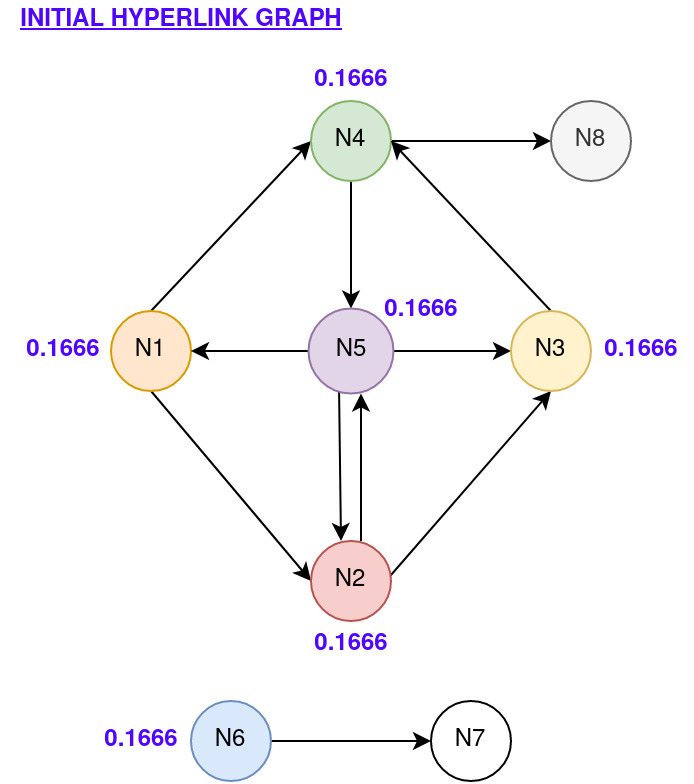
\includegraphics[scale=0.35]{imgs/initial.jpg}
\end{figure}
\begin{lstlisting}[language=bash,title={Initial PageRank}]
('n1', 0.16666666666666666)
('n2', 0.16666666666666666)
('n3', 0.16666666666666666)
('n4', 0.16666666666666666)
('n5', 0.16666666666666666)
('n6', 0.16666666666666666)
\end{lstlisting}
\begin{figure}[H]
    \centering
    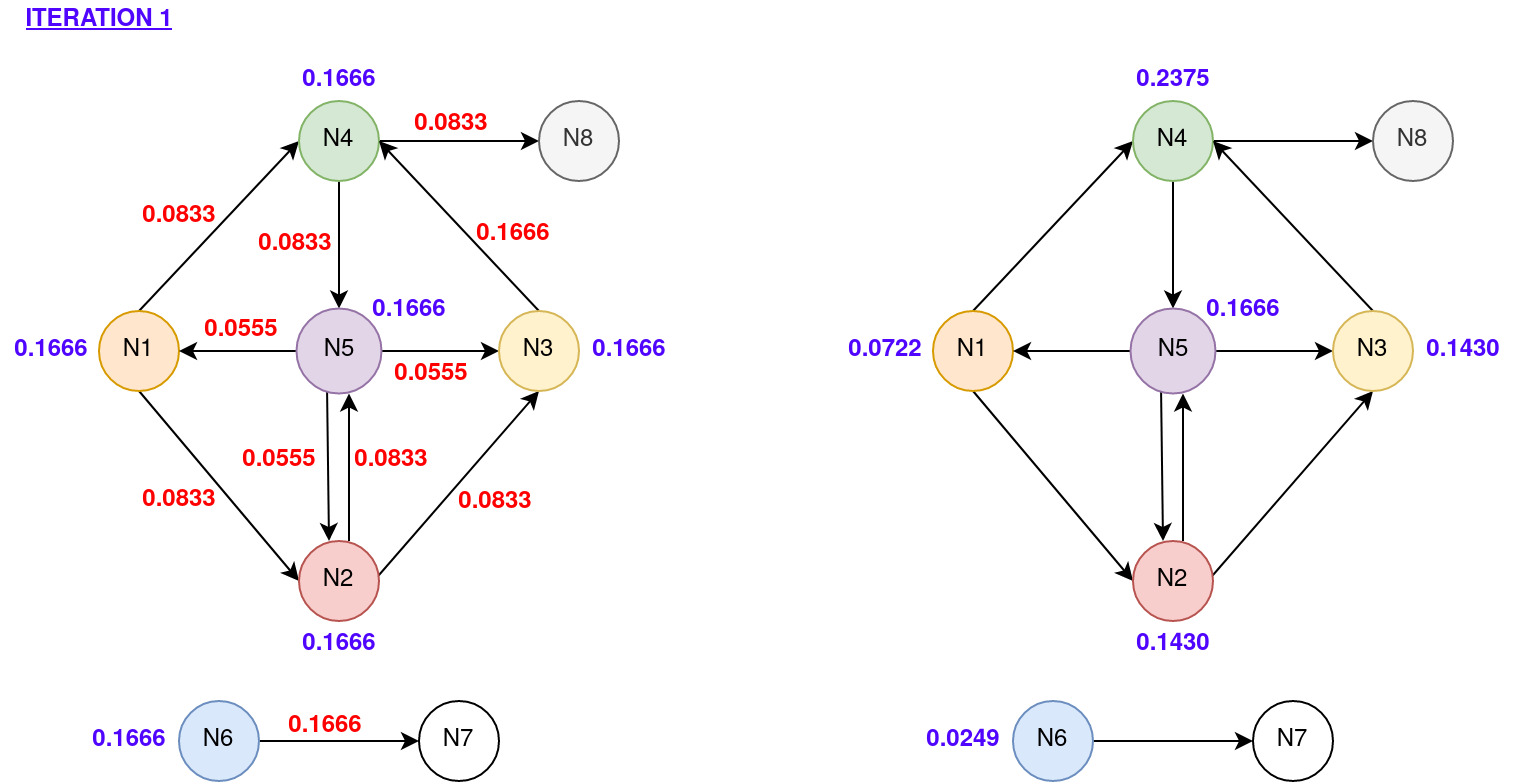
\includegraphics[scale=0.26]{imgs/iteration-1.jpg}
\end{figure}
\begin{minipage}{.45\textwidth}
\begin{lstlisting}[language=bash,title={Contributions}]
('n2', 0.08333333333333333)
('n4', 0.08333333333333333)
('n1', 0.05555555555555555)
('n2', 0.05555555555555555)
('n3', 0.05555555555555555)
('n7', 0.16666666666666666)
('n5', 0.08333333333333333)
('n8', 0.08333333333333333)
('n3', 0.08333333333333333)
('n5', 0.08333333333333333)
('n4', 0.16666666666666666)
\end{lstlisting}
\end{minipage}\hfill
\begin{minipage}{.45\textwidth}
\begin{lstlisting}[language=bash,title={New PageRanks}]
('n5', 0.16666666666666666)
('n8', 0.09583333333333333)
('n1', 0.07222222222222222)
('n4', 0.2375)
('n2', 0.14305555555555555)
('n3', 0.14305555555555555)
('n7', 0.16666666666666666)
('n6', 0.024999999999999998)
\end{lstlisting}
\end{minipage}
\begin{figure}[H]
    \centering
    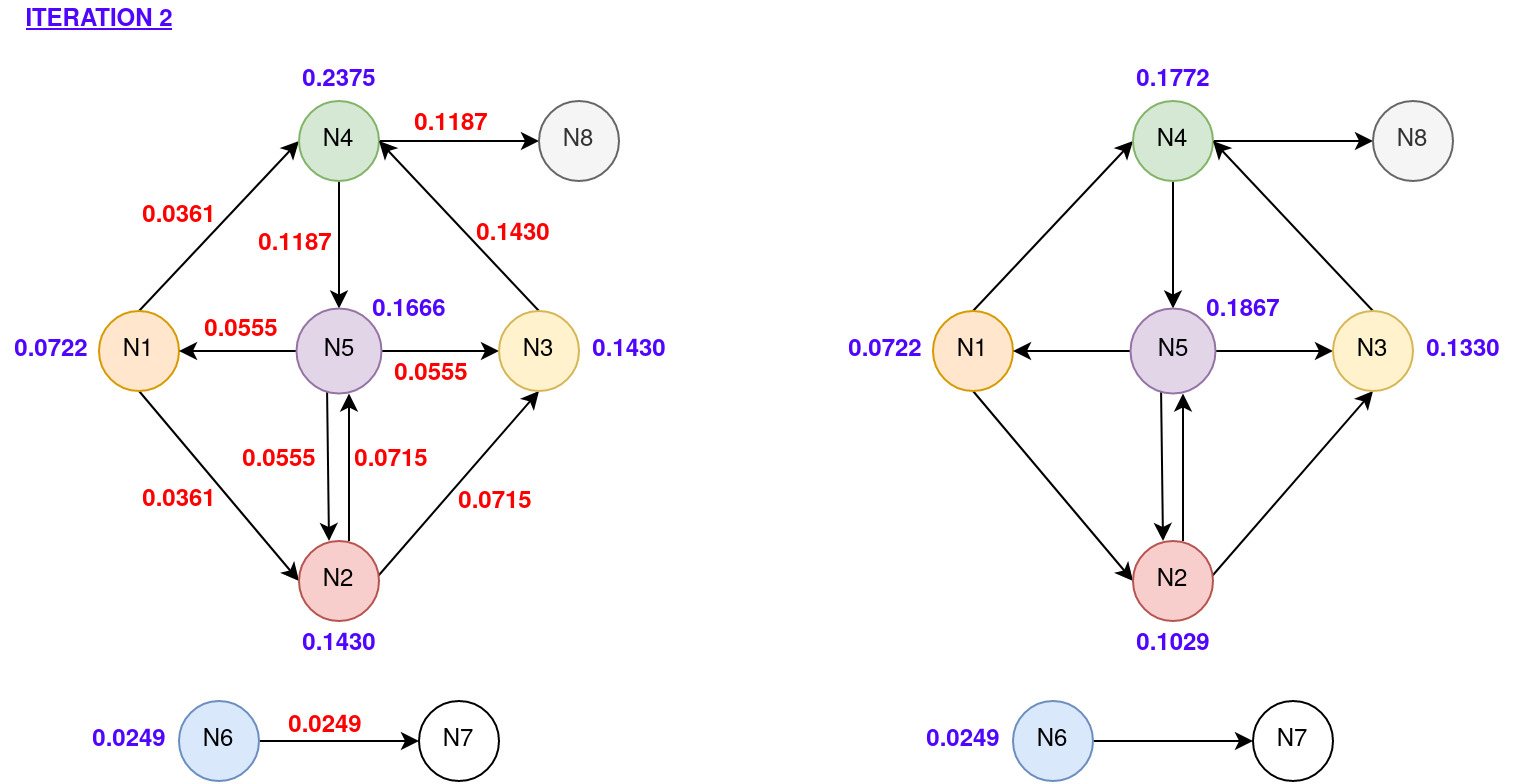
\includegraphics[scale=0.26]{imgs/iteration-2.jpg}
\end{figure}
\begin{minipage}{.45\textwidth}
\begin{lstlisting}[language=bash,title={Contributions}]
('n7', 0.024999999999999998)
('n3', 0.07152777777777777)
('n5', 0.07152777777777777)
('n1', 0.05555555555555555)
('n2', 0.05555555555555555)
('n3', 0.05555555555555555)
('n5', 0.11875)
('n8', 0.11875)
('n4', 0.14305555555555555)
('n2', 0.03611111111111111)
('n4', 0.03611111111111111)
\end{lstlisting}
\end{minipage}\hfill
\begin{minipage}{.45\textwidth}
\begin{lstlisting}[language=bash,title={New PageRanks}]
('n8', 0.1259375)
('n7', 0.04625)
('n2', 0.10291666666666666)
('n5', 0.1867361111111111)
('n4', 0.17729166666666663)
('n3', 0.13302083333333334)
('n1', 0.07222222222222222)
('n6', 0.024999999999999998)
\end{lstlisting}
\end{minipage}
\begin{figure}[H]
    \centering
    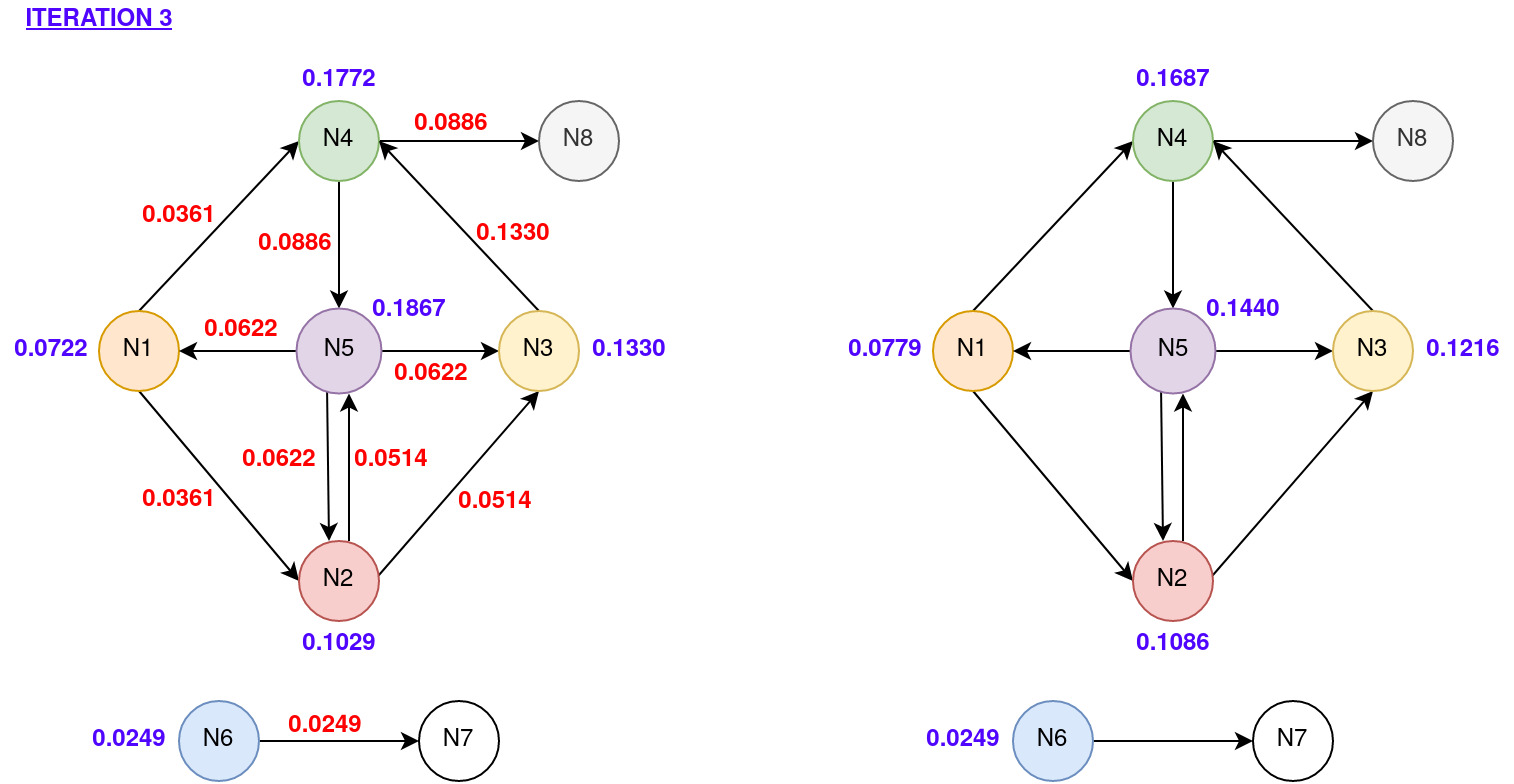
\includegraphics[scale=0.26]{imgs/iteration-3.jpg}
\end{figure}
\begin{minipage}{.45\textwidth}
\begin{lstlisting}[language=bash,title={Contributions}]
('n5', 0.08864583333333331)
('n8', 0.08864583333333331)
('n2', 0.03611111111111111)
('n4', 0.03611111111111111)
('n4', 0.13302083333333334)
('n1', 0.06224537037037037)
('n2', 0.06224537037037037)
('n3', 0.06224537037037037)
('n3', 0.05145833333333333)
('n5', 0.05145833333333333)
('n7', 0.024999999999999998)
\end{lstlisting}
\end{minipage}\hfill
\begin{minipage}{.45\textwidth}
\begin{lstlisting}[language=bash,title={New PageRanks}]
('n4', 0.16876215277777779)
('n7', 0.04625)
('n8', 0.10034895833333331)
('n1', 0.07790856481481481)
('n3', 0.12164814814814813)
('n5', 0.14408854166666665)
('n2', 0.10860300925925924)
('n6', 0.024999999999999998)
\end{lstlisting}
\end{minipage}\\
\\
Once both implementations and the debugging stage was concluded, the first and foremost validation we performed consisted in comparing the PageRank computation results produced by the Hadoop and Spark implementations. Having obtained the same exact output on this synthetic test dataset is by no means a rigorous validation, however it is a beginning.
\subsection{\texttt{wiki-micro.txt} dataset}
Finally both implementations were executed on the given \texttt{wiki-micro.txt} real world dataset. This allowed for observing the convergence of the PageRank computation. In an execution with $10$ iterations on a hyperlink graph made up of $2282$ nodes, convergence was reached after a few iterations. This is consistent with what found in the original PageRank paper: "\textit{on a $322$ million link database convergence to a reasonable tolerance in obtained in roughly $52$ iterations}".
\end{document}